\chapter[Metodologia]{Metodologia}
\label{metodologia}
Neste capítulo, detalha-se a implementação do módulo Nahid em linguagem de descrição de Hardware SystemVerilog. Este  módulo de detecção em hardware é basicamente a implementação da formulação dos passos da correlação proposta (Figura \ref{fig01}), utilizando uma \textit{FPGA}. Para isso, é necessário adequar  as operações para os componentes que estão disponíveis e foram escolhidos para realizar a computação de uma dada operação.  Além disso, para otimizar o tempo de resposta é necessário uma organização dessas operações em ciclos de \textit{clock}, para ter uma referência de tempo  para cada computação realizada e assim organizar a sequência das operações. Com isso , a arquitetura de detecção de ataques é proposta com o nome de Nahid. Essa arquitetura possui componentes de diversos níveis, nos quais estão dispostos dependendo da operação que esteja sendo feita no momento, vale ressaltar que essas operações são aritméticas, mudança no tamanho da palavra, registro e seleção. Segue abaixo as operações que o módulo em hardware realiza para efetuar a detecção de ataques.

Para o módulo de correlação em \textit{hardware} receber as instâncias de tráfego no trabalho \cite{HOQUE201748}, foi implementado  um módulo  chamado de pré-processador e ao final da computação, o módulo de hardware envia para outro módulo que irá realizar algum tratamento no sistema, chamado de gerenciador de segurança. Nota-se que os módulos do pré-processador e do gerenciador de segurança são implementados separadamente usando \textit|{software}. As máquinas que implementam esses módulos e o \textit{FPGA} podem comunicar-se usando as interfaces de E/S de alta velocidade suportadas pelos \textit{FPGAs} modernos, como \textit{PCI} e \textit{Ethernet}. O módulo de detecção de ataque recebe a instância de tráfego do módulo pré-processador. Além disso, ele recebe o perfil normal e um valor limiar do banco de dados do perfil criado pelo gerenciador de segurança. Cada uma das instâncias de tráfego e o perfil normal são vetores que consistem em três recursos de tráfego. O módulo de detecção de ataque calcula primeiro o NaHiD VERC entre a instância de tráfego de entrada e o perfil normal. O valor de correlação calculado é comparado com o limite para classificar a ocorrência de tráfego recebido como ataque ou normal. O resultado da classificação é armazenado no banco de dados \textit{log} para análise \textit{off-line} pelo gerenciador de segurança. Além disso, um alarme é gerado no caso de a instância ser classificada como um ataque.

\begin{figure}[H]
	\centering
	\caption{Operações que o Módulo em \textit{hardware} efetua}
	\subfloat[Calculos da correlação na forma aritmética]{
		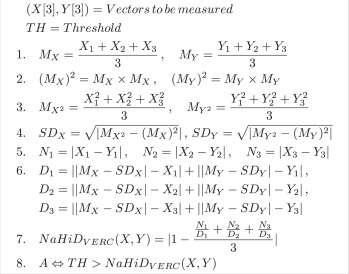
\includegraphics[height=5cm]{figures/Op1.jpg}
		\label{figdroopy}
	}
	\quad %espaco separador
	\subfloat[Calculos da correlação na forma de operações em \textit{hardware}]{
		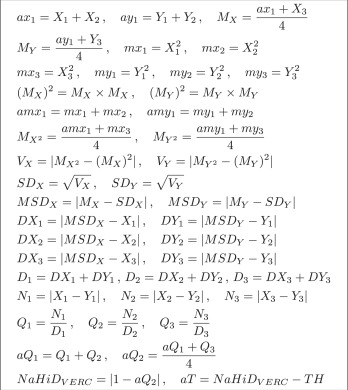
\includegraphics[height=5cm]{figures/Op2.jpg}
		\label{figsnoop}
		
		
	}
	\\{Fonte:\url{http://www.sciencedirect.com/science/article/pii/S0140366416306442}}
	\label{fig01}
\end{figure}

\section{Módulo Nahid}\label{Sub:equa}

Nahid é o componente de mais alto nível, sendo ele quem recebe as entradas(perfil normal e instâncias de tráfego em análise) do módulo pré-processador e envia a saída (resultado da análise) para o gerenciador de segurança. O Nahid é composto basicamente por dois componentes  internos, são esses: Datapath e Controller.  Além dos vetores de entrada citados anteriormente, o componente  Nahid recebe os sinais de controle, \textit{clock} e \textit{start} (que são os sinais que indicaram o início da detecção e as mudanças de ciclos). Esse componente  abstrai toda a combinação lógica que foi implementado nos componentes  internos, sendo este de suma importância para realizar a junção de entradas e saídas entre componentes internos, módulos e  gerenciadores. O código do módulo Nahid está no apêndice \ref{nahidcode}.
\begin{figure}[H]
	\label{ops}
	\centering
	\caption{Módulo Nahid}
	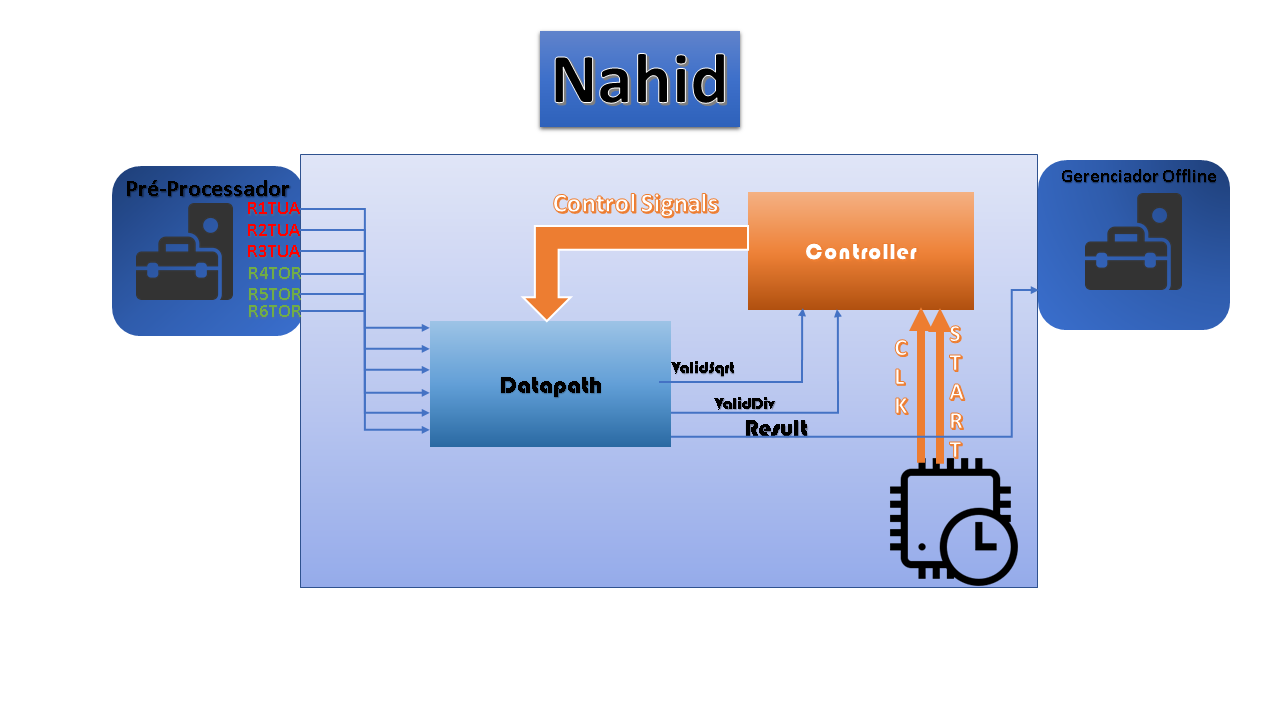
\includegraphics[width=12cm]{figures/NahidModule.png}\\
	{Fonte: Elaborada pelo autor}
\end{figure}

\subsection{Datapath}

O componente responsável por alocar todos os componentes que realizam as operações da detecção  é o Datapath. Por isso, o mesmo comporta no mínimo um dos componentes de mais baixo nível, que serão descritos posteriormente. O Datapath recebe os vetores de entradas(perfil normal e instâncias de tráfego em análise) do Nahid, pois esses dados são selecionados, tratados e registrados pelos componentes internos do Datapath. Porém para isso é necessário que seja indicado ao componente quais são as entradas a serem processadas num dado ciclo, por isso o Datapath recebe como entrada seletores provindos do Controller . Entretanto , o Datapath possui saídas para o controller, pois em alguns ciclos é necessário de alguma confirmação de algum componente  interno ao Datapath, além disso a saída do sistema será um resultado registrado num componente interno e será em enviado ao componente de mais alto nível (Nahid). Segue abaixo, uma breve explicação de cada componente do Datapath. O código do Datapath está no apêndice \ref{codedatapath}.


\begin{figure}[H]
	\centering
	\caption{Design do Datapath desenvolvido por \cite{HOQUE201748}}
	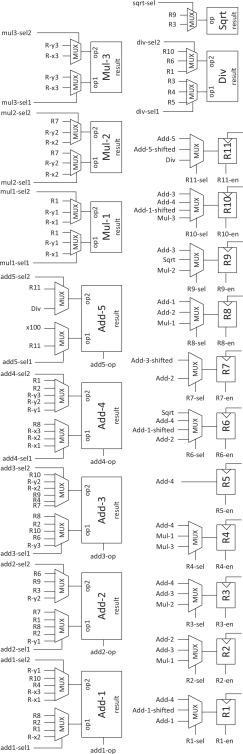
\includegraphics[width=8cm]{figures/dp.jpg}\\
	{Fonte:\url{http://www.sciencedirect.com/science/article/pii/S0140366416306442}}
	\label{extend}
\end{figure}



\subsubsection{Extend}
Esse componente possui a função de estender o tamanho de uma palavra de bits de qualquer tamanho (menor que 23), para uma palavra de mesmo conteúdo com tamanho de 23 bits. Basicamente, ele completa com 0's o a esquerda da palavra, até o tamanho desta ser de 23 bits.Esse componente é de suma importância nas operações de soma, uma vez que o componentes de soma Adder  possuem entradas de tamanho de 23 bits. O Datapath possui 12 componentes do tipo extend. Esse componente é do tipo de mudança no tamanho da palavra e em um ciclo ele completa sua computação. O código do componente extende está no apêndice \ref{codeextend}.


\begin{figure}[H]
	\centering
	\caption{Componente extend}
	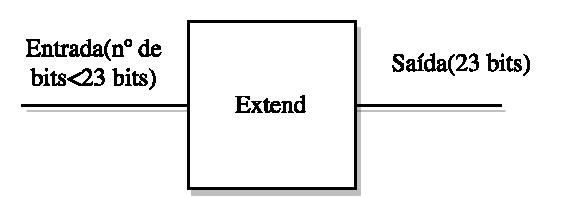
\includegraphics[width=6cm]{figures/Extend.pdf}\\
	
	{Fonte: Elaborada pelo autor}
	\label{extend}
\end{figure}


\subsubsection{Reduce}
Esse componente possui a função de reduzir o tamanho de uma palavra de bits de qualquer tamanho (maior que 11), para uma palavra de mesmo conteúdo com tamanho de 11 bits. Basicamente, ele pega os 11 bits mais significativos da palavra. Esse componente é de suma importância nas operações de multiplicação, uma vez que o componentes de multiplicação( Mul) possuem entradas de tamanho de 11 bits. O Datapath possui 4 componentes do tipo reduce. Esse componente é do tipo de mudança no tamanho da palavra e um em ciclo ele completa sua computação. O código do componente extende está no apêndice \ref{codereduce}.


\begin{figure}[H]
	\centering
	\caption{Componente Reduce}
	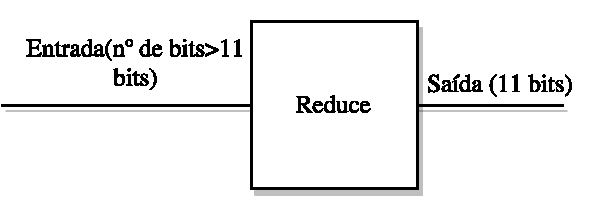
\includegraphics[width=6cm]{figures/Reduce.pdf}\\
	
	{Fonte: Elaborada pelo autor}
	\label{reduce}
\end{figure}


\subsubsection{Mux}
Esse componente possui a função de ter na entrada vários opções, porém a cada iteração, existe um seletor que indica que entrada será utilizada num dado momento, levando para saída do componente essa escolha. Esse componente é de suma importância para reutilização de componentes, deixando a arquitetura mais enxuta e coesa, sendo muito utilizado no Controller, pois para cada ciclo existem determinadas escolhas nesses multiplexadores. É importante ressaltar, que no Datapath existem mux de diversos tamanhos (2 entradas,4 entradas e 6 entradas), isso está diretamente relacionado com o componente que recebe a saída do mux, pois quanto mais ele pode ser utilizado por entradas diferentes, maior será o número de entradas no multiplexador combinado a esse componente. Devido aos multiplexadores terem grande importância na reutilização de componentes, existem duas principais frentes de alocação de mux no Datapath. Nas operações aritméticas(Multiplicadores e Somadores) e de registro(Registradores). Esse componente é do tipo de seleção de dados e em um ciclo ele completa sua computação. O código do componente mux está no apêndice \ref{codemux}.	

\begin{figure}[H]
	\caption{Tipos do componente Mux no módulo 	}
	\centering
	\subfloat[Mux2]{
		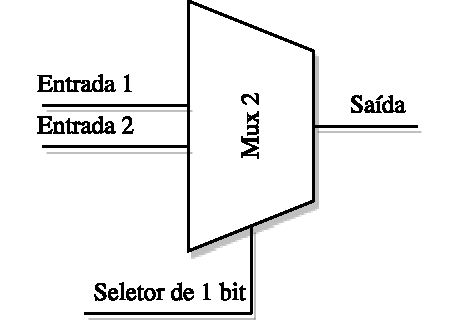
\includegraphics[height=4cm]{figures/Mux2.pdf}
		\label{figdroopy}
	}
	\quad %espaco separador
	\subfloat[Mux4]{
		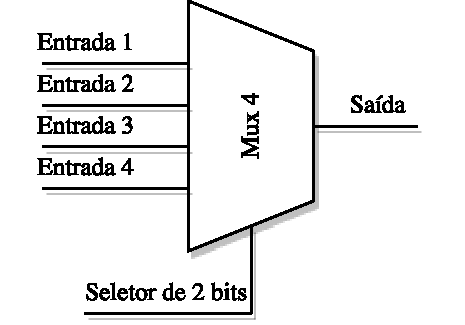
\includegraphics[height=4cm]{figures/Mux4.pdf}
		\label{figsnoop}
	}
	\quad %espaco separador
	\subfloat[Mux6]{
		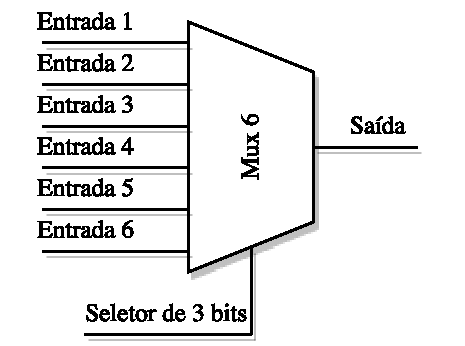
\includegraphics[height=4cm]{figures/Mux6.pdf}
		\label{figsnoop}
	}
	
	{Fonte: Elaborada pelo autor}
	\label{fig01}
\end{figure}

\subsubsection{Mul}
Esse componente possui a função de receber duas entradas, e realizar a multiplicação aritmética das mesmas, gerando uma saída do resultado. Foi utilizado um mul que recebe entradas de 11 bits podendo gerar até 22 bits no resultado dessa multiplicação. Existem 3 multiplicadores no Datapath, que em nosso módulo realizam operação de quadrado de um número, ou seja as multiplicações tem as mesmas entradas num dado momento. Esse componente é do tipo operações aritméticas e em um ciclo ele completa sua computação. O código do componente mul está no apêndice \ref{codemul}.

\begin{figure}[H]
	\centering
	\caption{Componente Mul}
	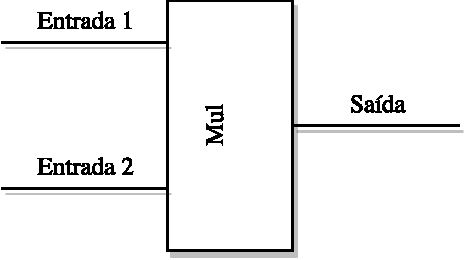
\includegraphics[width=6cm]{figures/Mul.pdf}\\
	
	{Fonte: Elaborada pelo autor}
	\label{Mul}
\end{figure}



\subsubsection{Adder}
Esse componente possui a função de receber duas entradas, e realizar a soma aritmética das mesmas, gerando uma saída do resultado. Foi utilizado um adder que recebe entradas de 23 bits podendo gerar até 24 bits no resultado dessa soma. Vale ressaltar que o componente possui 4 modos de operação, o que caracteriza diferentes formas de somar as entradas. Esses modos são:
\begin{itemize}
	\item O modo 0: A soma padrão de dois números positivos.
	\item O modo 1: A soma de dois números positivos, com o resultado dividido por 4.
	\item O modo 2: O módulo de dois números positivos
	\item O modo 3: O módulo de dois números positivos, com o resultado dividido por 4.
\end{itemize}

Esses modos de operação, são necessários pelos diversos “cálculos” que são necessários na formulação da correlação que o módulo implementa, por isso  é necessário que algum componente implemente essas adições, sendo escolhido o Somador.
Existem 5 somadores no Datapath, que no módulo realizam operações de adição necessárias. Vale ressaltar que o seletor de operação, também é uma entrada do adder. Esse componente é do tipo operações aritméticas e em um ciclo ele completa sua computação. O código do componente adder está no apêndice \ref{codeadder}.

\begin{figure}[H]
	\centering
	\caption{Componente Adder}
	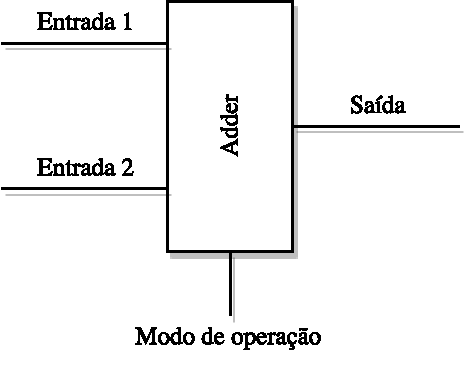
\includegraphics[width=6cm]{figures/Adder.pdf}\\
	
	{Fonte: Elaborada pelo autor}
	\label{adder}
\end{figure}

\subsubsection{Divider}
Esse componente possui a função de receber duas entradas, e realizar a divisão aritmética das mesmas, gerando uma saída do resultado. Esse componente possui certas peculiaridades, pois uma divisão em hardware é mais custosa, pela existência de números fracionários nos resultados de divisões decimais, que interferem diretamente nas operações e no resultado do módulo. Por isso existe a necessidade da utilização de alguma representação numérica que possa trazer resultados fracionários, foi utilizado nesse caso representação em ponto fixo como falado anteriormente. O componente Divider utilizado foi o IP core da \textit{xilinx “Divider Generator”}, que foi configurado da seguinte forma: 
\begin{itemize}
	\item 	Dividendo: 12 bits
	\item 	Divisor: 12 bits
	\item 	Quociente: 12 bits
	\item 	Parte Fracionária: 8 bits
\end{itemize}
Em outras palavras, temos 2 entradas de 12 bits e uma saída de 20 bits, porém na representação de ponto fixa, tem-se 12.8(12 números na parte inteira e 8 na decimal). Além dessas instâncias, existem dois sinais de controle no módulo, o \textit{"valid in"} (responsável por indicar que o componente está pronto para receber as entradas e iniciar a computação) e o \textit{"valid out"} (responsável por indicar que o componente acabou de realizar a operação por completo e já tem o resultado), esses sinais são de suma importância para a organização do módulo e regulação dos ciclos. Existe apenas um componente do tipo do Divider, que realiza divisões que não possuem divisor diferente de potências de 2 (pois pode-se utilizar mecanismos mais simples, para realizar essas divisões, mantendo o resultado no universo dos inteiros).  Esse componente é do tipo operações aritméticas e em 22 ciclos ele completa sua computação.

\begin{figure}[H]
	\centering
	\caption{Componente Divider}
	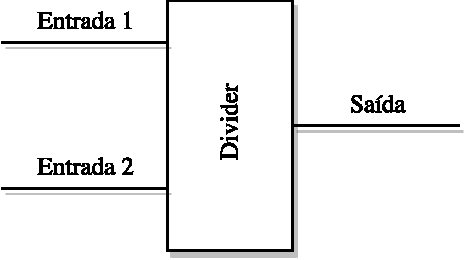
\includegraphics[width=6cm]{figures/Divider.pdf}\\
	
	{Fonte: Elaborada pelo autor}
	\label{divider}
\end{figure}

\subsubsection{Sqrt}
Esse componente possui a função de receber uma entrada, e realizar a raiz quadrada aritmética da mesma, gerando uma saída do resultado. Esse componente possui resultados inteiros, porém o resultado é um inteiro aproximado para números que não possuem raízes fechadas, pois é possível os números de entradas não serem quadrados perfeitos e o resultado da raiz ser número com casas decimais. Para realizar a busca e aproximação de resposta, é necessário algum algoritmo de busca dessa raiz, gerando um certo custo de ciclos, como no divisor. Para tal o componente \textit{sqrt} utilizado foi o \textit{IP core} da \textit{xilinx “Cordic”} (função Raiz), que foi configurado da seguinte forma: 
\begin{itemize}
	\item Entrada: 22 bits
	\item Saída: 12 bits
\end{itemize}
Logo, temos 1 entrada de 22 bits e uma saída de 12 bits. Além dessas instâncias, existem dois sinais de controle no módulo, o \textit{"valid in"} (responsável por indicar que o componente está pronto para receber a entrada e iniciar a computação) e o \textit{"valid out"} (responsável por indicar que o componente acabou de realizar a operação por completo e já tem o resultado), esses sinais são de suma importância para a organização do módulo e regulação dos ciclos. Existe apenas um componente do tipo do sqrt, esse componente é do tipo operações aritméticas e em 6 ciclos ele completa sua computação.

\begin{figure}[H]
	\centering
	\caption{Componente Sqrt}
	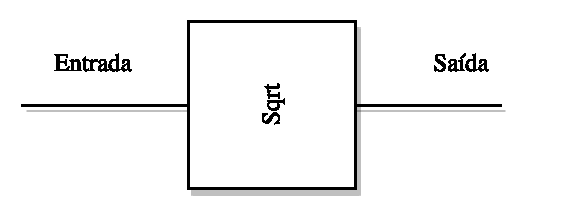
\includegraphics[width=6cm]{figures/sqrt.pdf}\\
	
	
	{Fonte: Elaborada pelo autor}
	\label{Sqrt}
\end{figure}

\subsubsection{Register}
Esse componente possui a função de receber uma entrada, e armazenar o valor recebido a partir da próxima subida do \textit{clock} e atualizar o valor que estiver na entrada na próxima subida do \textit{clock}. De forma que pelo menos durante um ciclo o registrador terá o valor recebido num dado momento, por isso podemos considerar o conjunto de registradores como a memória do módulo. Os registradores são de suma importância para a realizar as operações, uma vez que não para realizar todos os passos da correlação, “guardam-se” variáveis de uma operação para utilizar nas próximas operações. O Registrador implementado por padrão recebe entradas de 24 bits e a saída tem o mesmo tamanho, porém existem registradores específicos que possuem tamanhos diferentes do padrão, por serem usados para em fins específicos. Além da entrada, o Registrador recebe o sinal \textit{enable} (responsável para habilitar ou não o registro do componente, no próximo ciclo de \textit{clock}) e \textit{clr} (responsável por zerar o registro do componente, no próximo ciclo de \textit{clock}). Existem 11 registradores no Datapath, que realizam o registro necessários no módulo. Esse componente é do tipo registro e em um ciclo ele completa sua computação. O código do componente register está no apêndice \ref{coderegister}.

\begin{figure}[H]
	\centering
	\caption{Componente Register}
	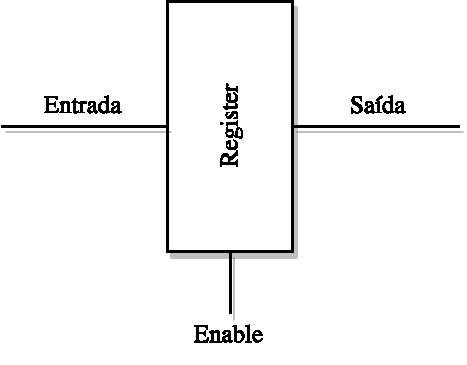
\includegraphics[width=6cm]{figures/Register.pdf}\\
	
	{Fonte: Elaborada pelo autor}
	\label{register}
\end{figure}

\subsection{Controller}
O componente responsável por organizar os ciclos das operações do Módulo Nahid é o Controller. Quais componentes do Datapath que serão utilizados num determinado ciclo de computação e em que ciclo teremos os resultados de uma dada operação, são as principais funções desse componente. Esse componente, utiliza o conceito de máquina de estados, para realizar uma computação cíclica e prática, afim dos cálculos serem realizados de forma otimizada. O Controller recebe o \textit{clk} (\textit{clock} do sistema) e o \textit{start} (sinal que indica o início do módulo) do Nahid, para que o componente garante que o sistema está síncrono. Além dessas entradas, como dito anteriormente, recebe os sinais \textit{“valid out”} dos componentes Divider e Sqrt. O Controller possui saídas para o Datapath, para indicar a esse componente o que será utilizado num dado ciclo. A estrutura do controller pode ser dividida em dois cases:
\begin{enumerate}
	\item Case de operações: Esse case é responsável por indicar todas as operações que serão feitos em todos os ciclos. 
	\item Case de transições de ciclos: Esse case é responsável por indicar quando haverá as transições de um ciclo para outro.
\end{enumerate} 

\begin{figure}[H]
	\centering
	\caption{Esquemático do controller,ciclos de entrada e saídas para as  entradas do datapath num dado  ciclo de \textit{clock}}
	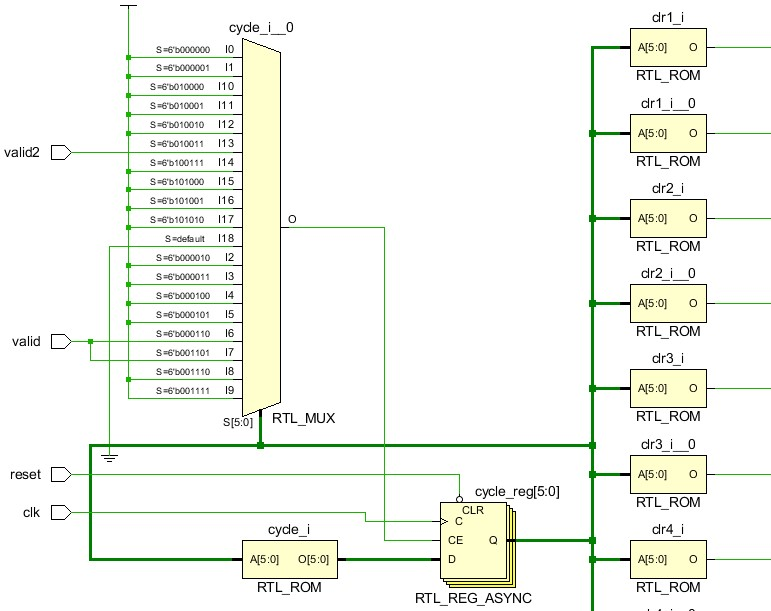
\includegraphics[width=10cm]{figures/controller.jpg}\\
	{Fonte: Elaborada pelo autor}	
	\label{ciclos}
\end{figure}

\begin{figure}[H]
	\centering
	\caption{Ciclos do Módulo Nahid  \ref{Tab:Tb}}
	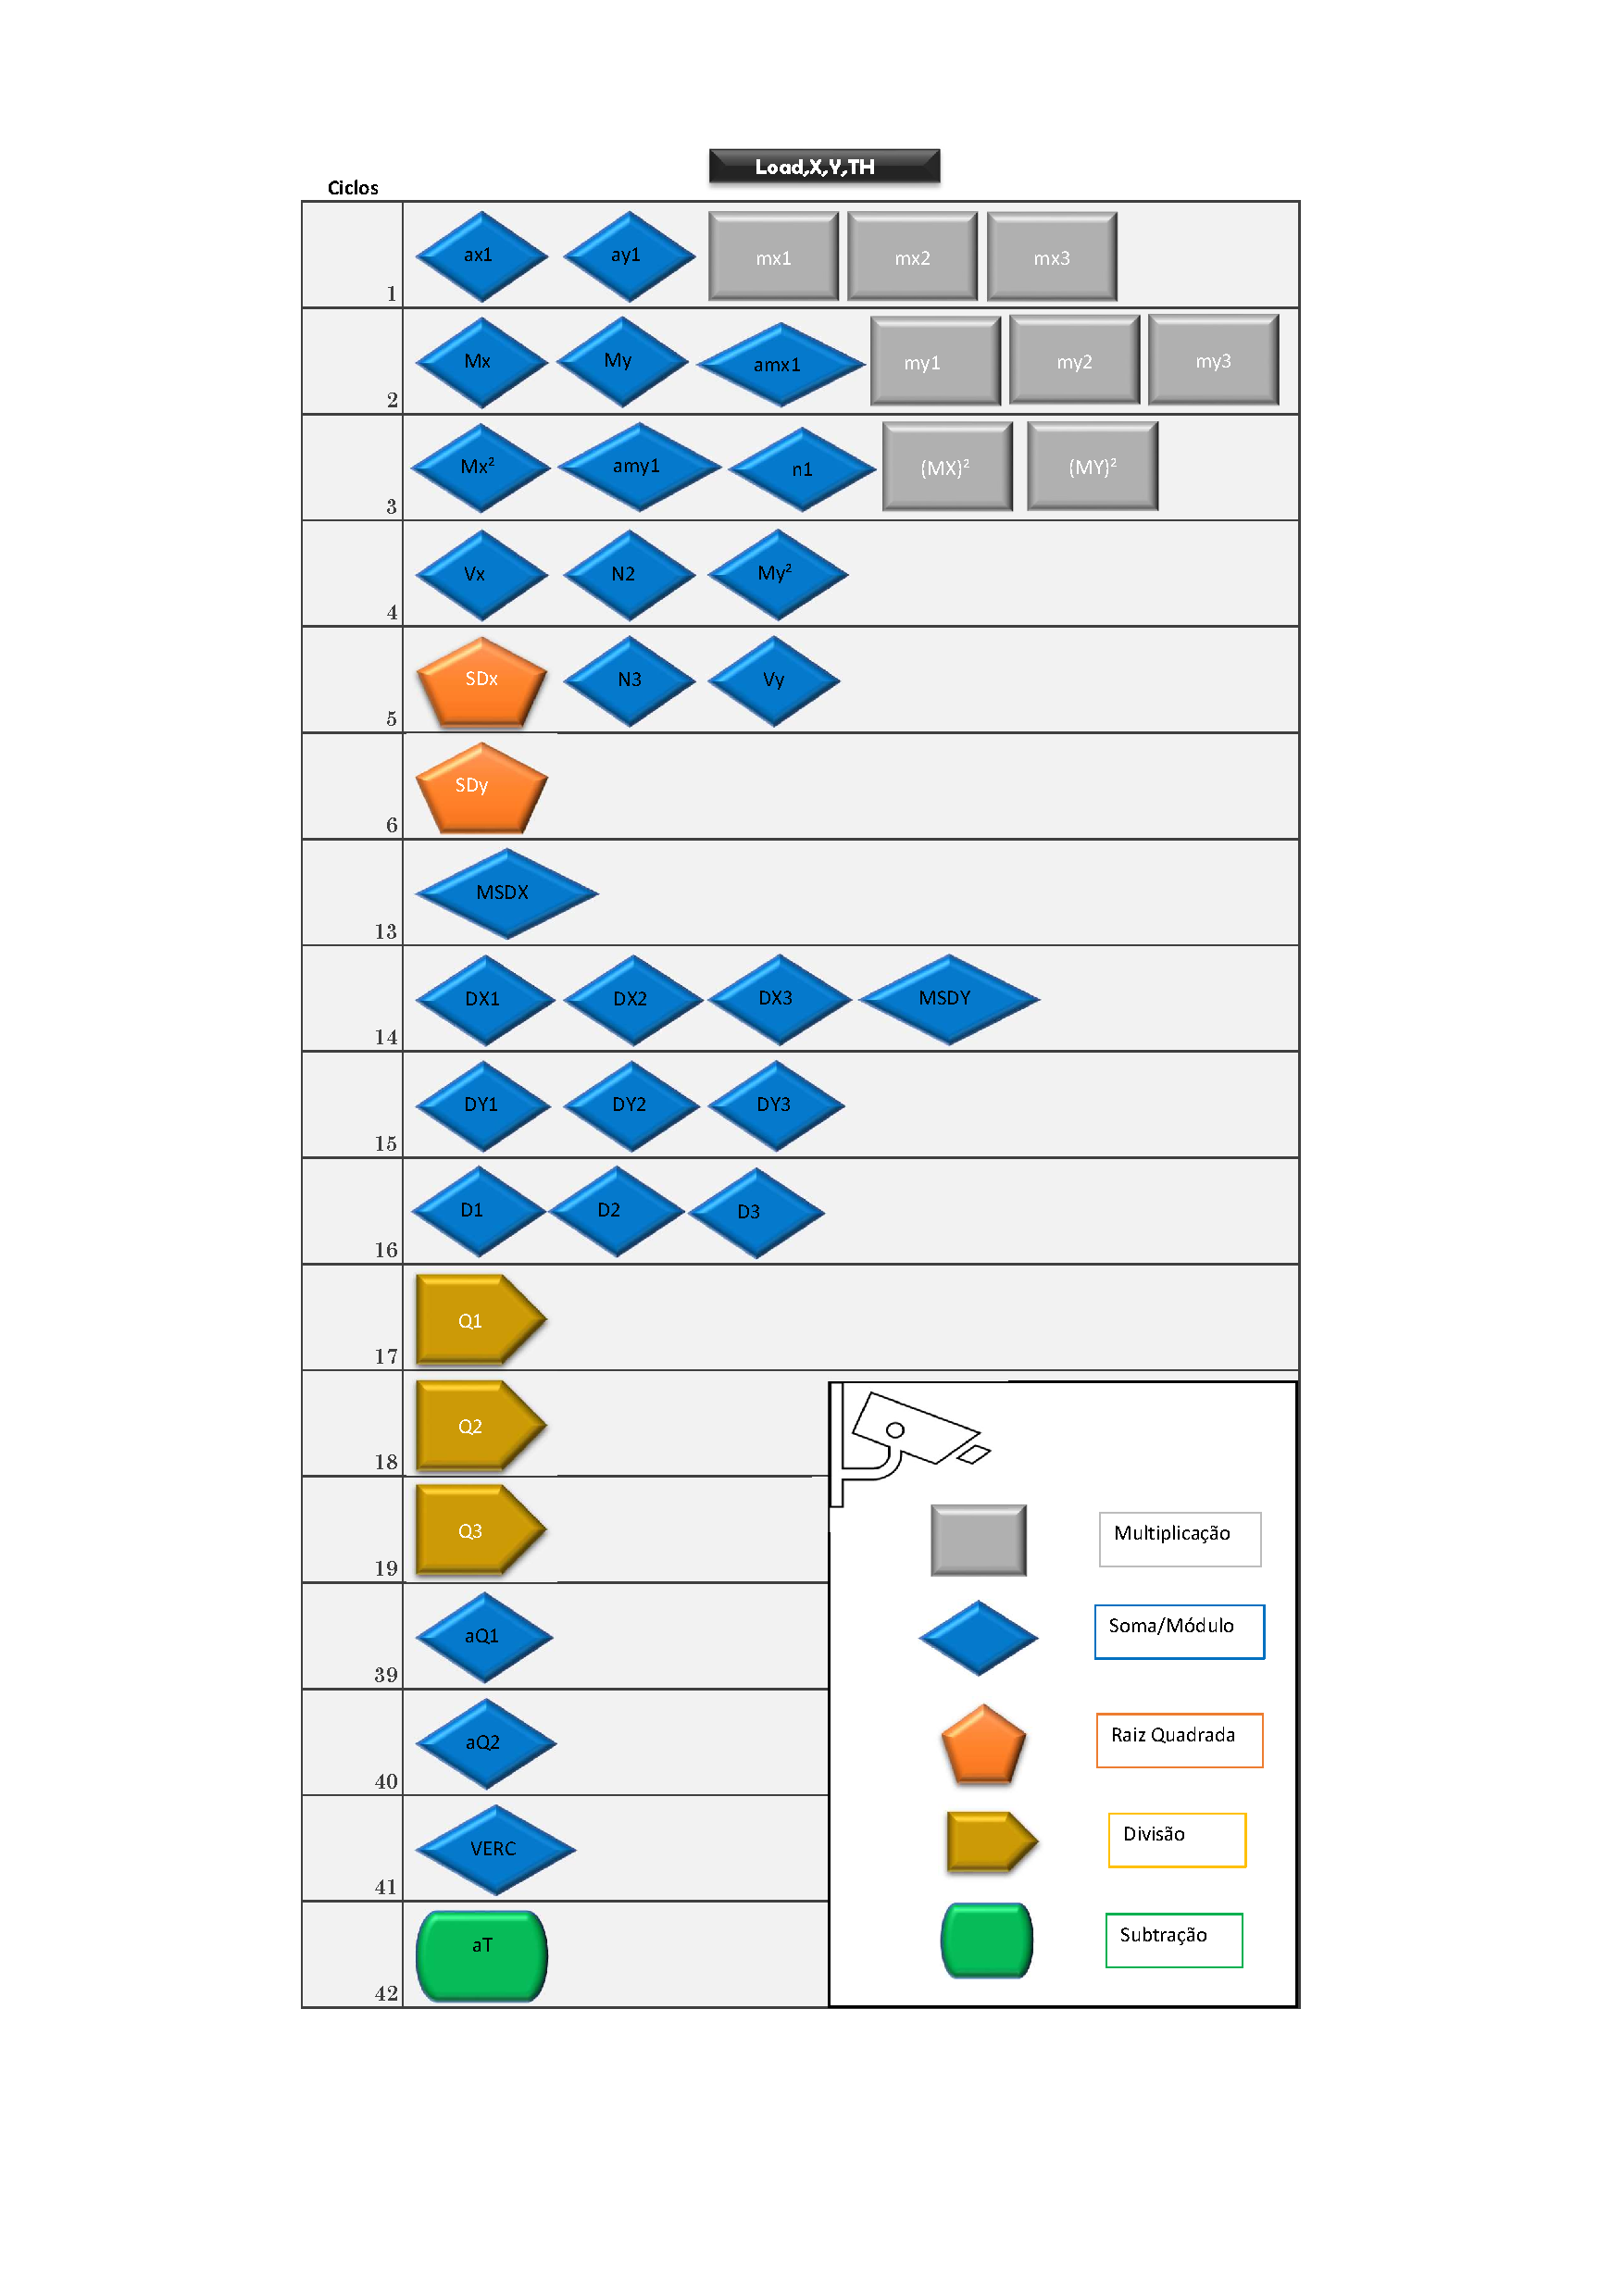
\includegraphics[width=12cm]{figures/TabelaCiclos.pdf}\\
	
	{Fonte: Elaborada pelo autor}
	\label{ciclos}
\end{figure}

A figura \ref{ciclos}, representa os ciclos que o módulo Nahid segue, para realizar a computação de detecção. Vale ressaltar que existem operações que possuem latência de vários ciclos de \textit{clock}. O código do Controller está no apêndice \ref{codecontroller}.